\title{Study Guide for Midterm 2 for Algebra-Based Physics: Electricity and Magnetism}
\author{Dr. Jordan Hanson - Whittier College Dept. of Physics and Astronomy}
\date{\today}
\documentclass[10pt]{article}
\usepackage[a4paper, total={18cm, 27cm}]{geometry}
\usepackage{outlines}
\usepackage{graphicx}
\usepackage{amsmath}
\begin{document}
\maketitle

\section{Equations and constants}

\begin{enumerate}
\item Kirchhoff's Rules: 1) $I_{in} + I_{out} = 0$ (Junction Rule) 2) $\sum_{loop} V_i = 0$ (Loop Rule)
\item Ohm's Law: $V = IR$
\item Power from current: $P=IV$
\item Voltage in an RC across the capacitor: $V(t) = \epsilon\left(1 - \exp\left(-t/\tau\right)\right)$, where $\epsilon$ is the battery voltage and $\tau = RC$.
\item Centripetal force: $F_C = mv^2/r$.
\item Magnetic torque: $\vec{\tau}_B = \vec{\mu} \times \vec{B}$
\item Magnitude of torque: $|\vec{\tau}_B| = \mu B \sin\theta$
\item Magnetic dipole moment: $\vec{\mu} = I \vec{A}$ (the current times the area vector)
\item Magnetic field at the center of a current-carrying loop: $\vec{B} = (\mu_0 I)/(2 R)\hat{z}$, if the current is in the x-y plane.
\item Magnetic field due to a current-carrying wire at a distance R: $B = (\mu_0 I)/(2 \pi R)$, right-hand rule gives direction.
\item Ampere's Law: $\int \vec{B} \cdot d\vec{s} = \mu_0 I_{enc}$ which is $B S = \mu_0 I_{enc}$ for simple cases where B is constant around the path.
\item Magnetic permeability: $\mu_0 = 4\pi \times 10^{-7}$ T m A$^{-1}$
\item The Hall Effect: $V_H = B l v$.
\end{enumerate}

\section{Exercises}

\begin{enumerate}
\item \textbf{Review Problem (similar exercise on the final)}
\begin{enumerate}
\item 
\begin{figure}[ht]
\centering
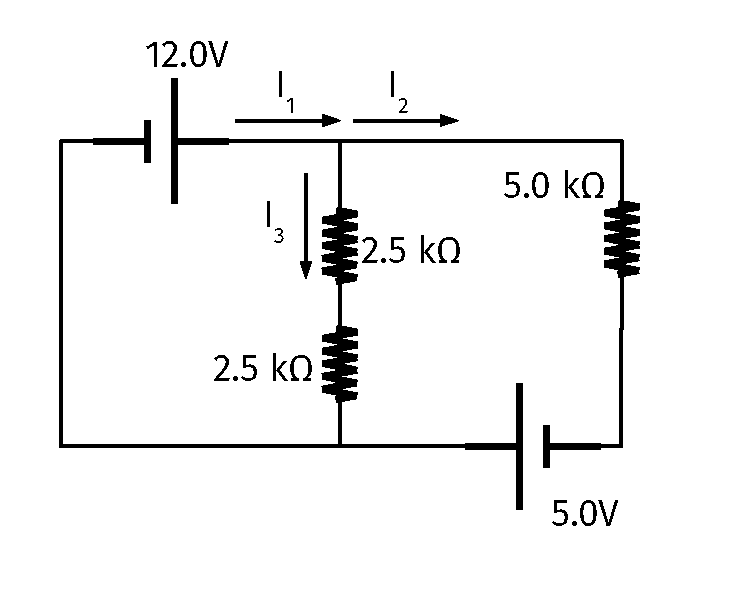
\includegraphics[width=0.4\textwidth]{iV.pdf}
\caption{\label{fig:circuit1} A circuit with three resistors.}
\end{figure}
Solve for the currents $I_1$-$I_3$ in Fig. \ref{fig:circuit1}. \\ $I_3 = 12/5$ mA, $I_2 = 17/5$ mA, and $I_1 = 29/5$ mA.
\end{enumerate} \clearpage
\item \textbf{Chapter 23: Magnetic Induction, Faraday's Law, and AC power}
\begin{enumerate}
\item
\begin{figure}
\centering
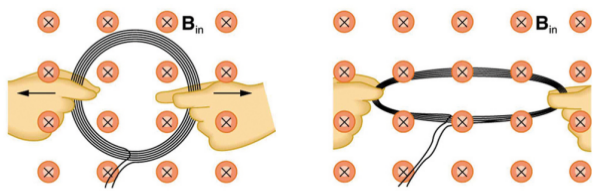
\includegraphics[width=0.6\textwidth]{flux1.png}
\caption{\label{fig:flux1} (Left) A magnetic field passes through loops of wire.  (Right) The loops are stretched, reducing the area.}
\end{figure}
In Fig. \ref{fig:flux1} (left) a uniform magnetic field passes through loops of wire.  In Fig. \ref{fig:flux1} (right) the \textbf{area} of the loops is reduced by stretching the loops.  Which of the following is true?
\begin{itemize}
\item A: No current flows through the wires.
\item B: Current does flow through the wires, but there is no induced emf in the wires.
\item C: Current flows through the wires, because the induced emf is caused by a change in electric flux.
\item D: Current flows through the wires, because the induced emf is caused by a change in magnetic flux.
\end{itemize}
(\textit{The answer is D. Magnetic flux $\phi = \vec{B} \cdot \vec{A} = BA$ in this case.  If the area changes, so does the flux.}
\end{enumerate}
\end{enumerate}
\end{document}